\documentclass{article}
\usepackage{graphicx} % Required for inserting images
\usepackage{hyperref}

\title{Methodology for Predictive calculator}
\author{Anton Mukin}
\date{June 2025}

\begin{document}

\maketitle

\section{Brief Summary of the Project}
This Matura project investigates and evaluates the arithmetic capabilities 
of different neural networks. 
\\
The project began with a literature review to 
generate a hypothesis regarding the weaknesses of neural networks in 
performing simple arithmetic. This literature review was submitted as the 
Zwischenprodukt, alongside a proof-of-concept notebook featuring a 
comparison of Feed-forward Neural Networks (FNNs) of different sizes.
\\
The next step was to build a Recurrent Neural Network (RNN) and similar 
attention-based RNNs to investigate their arithmetic capabilities and 
compare them to those of the FNN using a benchmark.
\\
The benchmark's baseline was defined to be the performance of a basic FNN's 
performance on different, but roughly still similar arithmetic tasks.
\\
Afterwards, the same was done for the transformer type of neural network 
model. Here, their exact functionality was thuroughly investigated, because 
of their unique architectures.
\\
Lastly a simillar workflow was repeated for some bigger, pre-trained models. 
\\
And finally all the findings were collected and evaluated as a whole.


\section{Introduction to this document}
The goal of this document is assisting reproducability and showing how the 
findings discussed in the other document have been obtained.
\\[2em]
All of the code written for this project is available in the github 
reporsitory: 
\\
\url{https://github.com/AntonStantan/matura}
\\
In this project all of the code is written in Python-notebooks (Jupyter Lab). 
\\
Most of the models were trained locally on a Nvidia GPU device: \it{Nvidia 
Jetson Orin Nano Super Developer Kit}

\begin{figure}[ht]
    \centering
    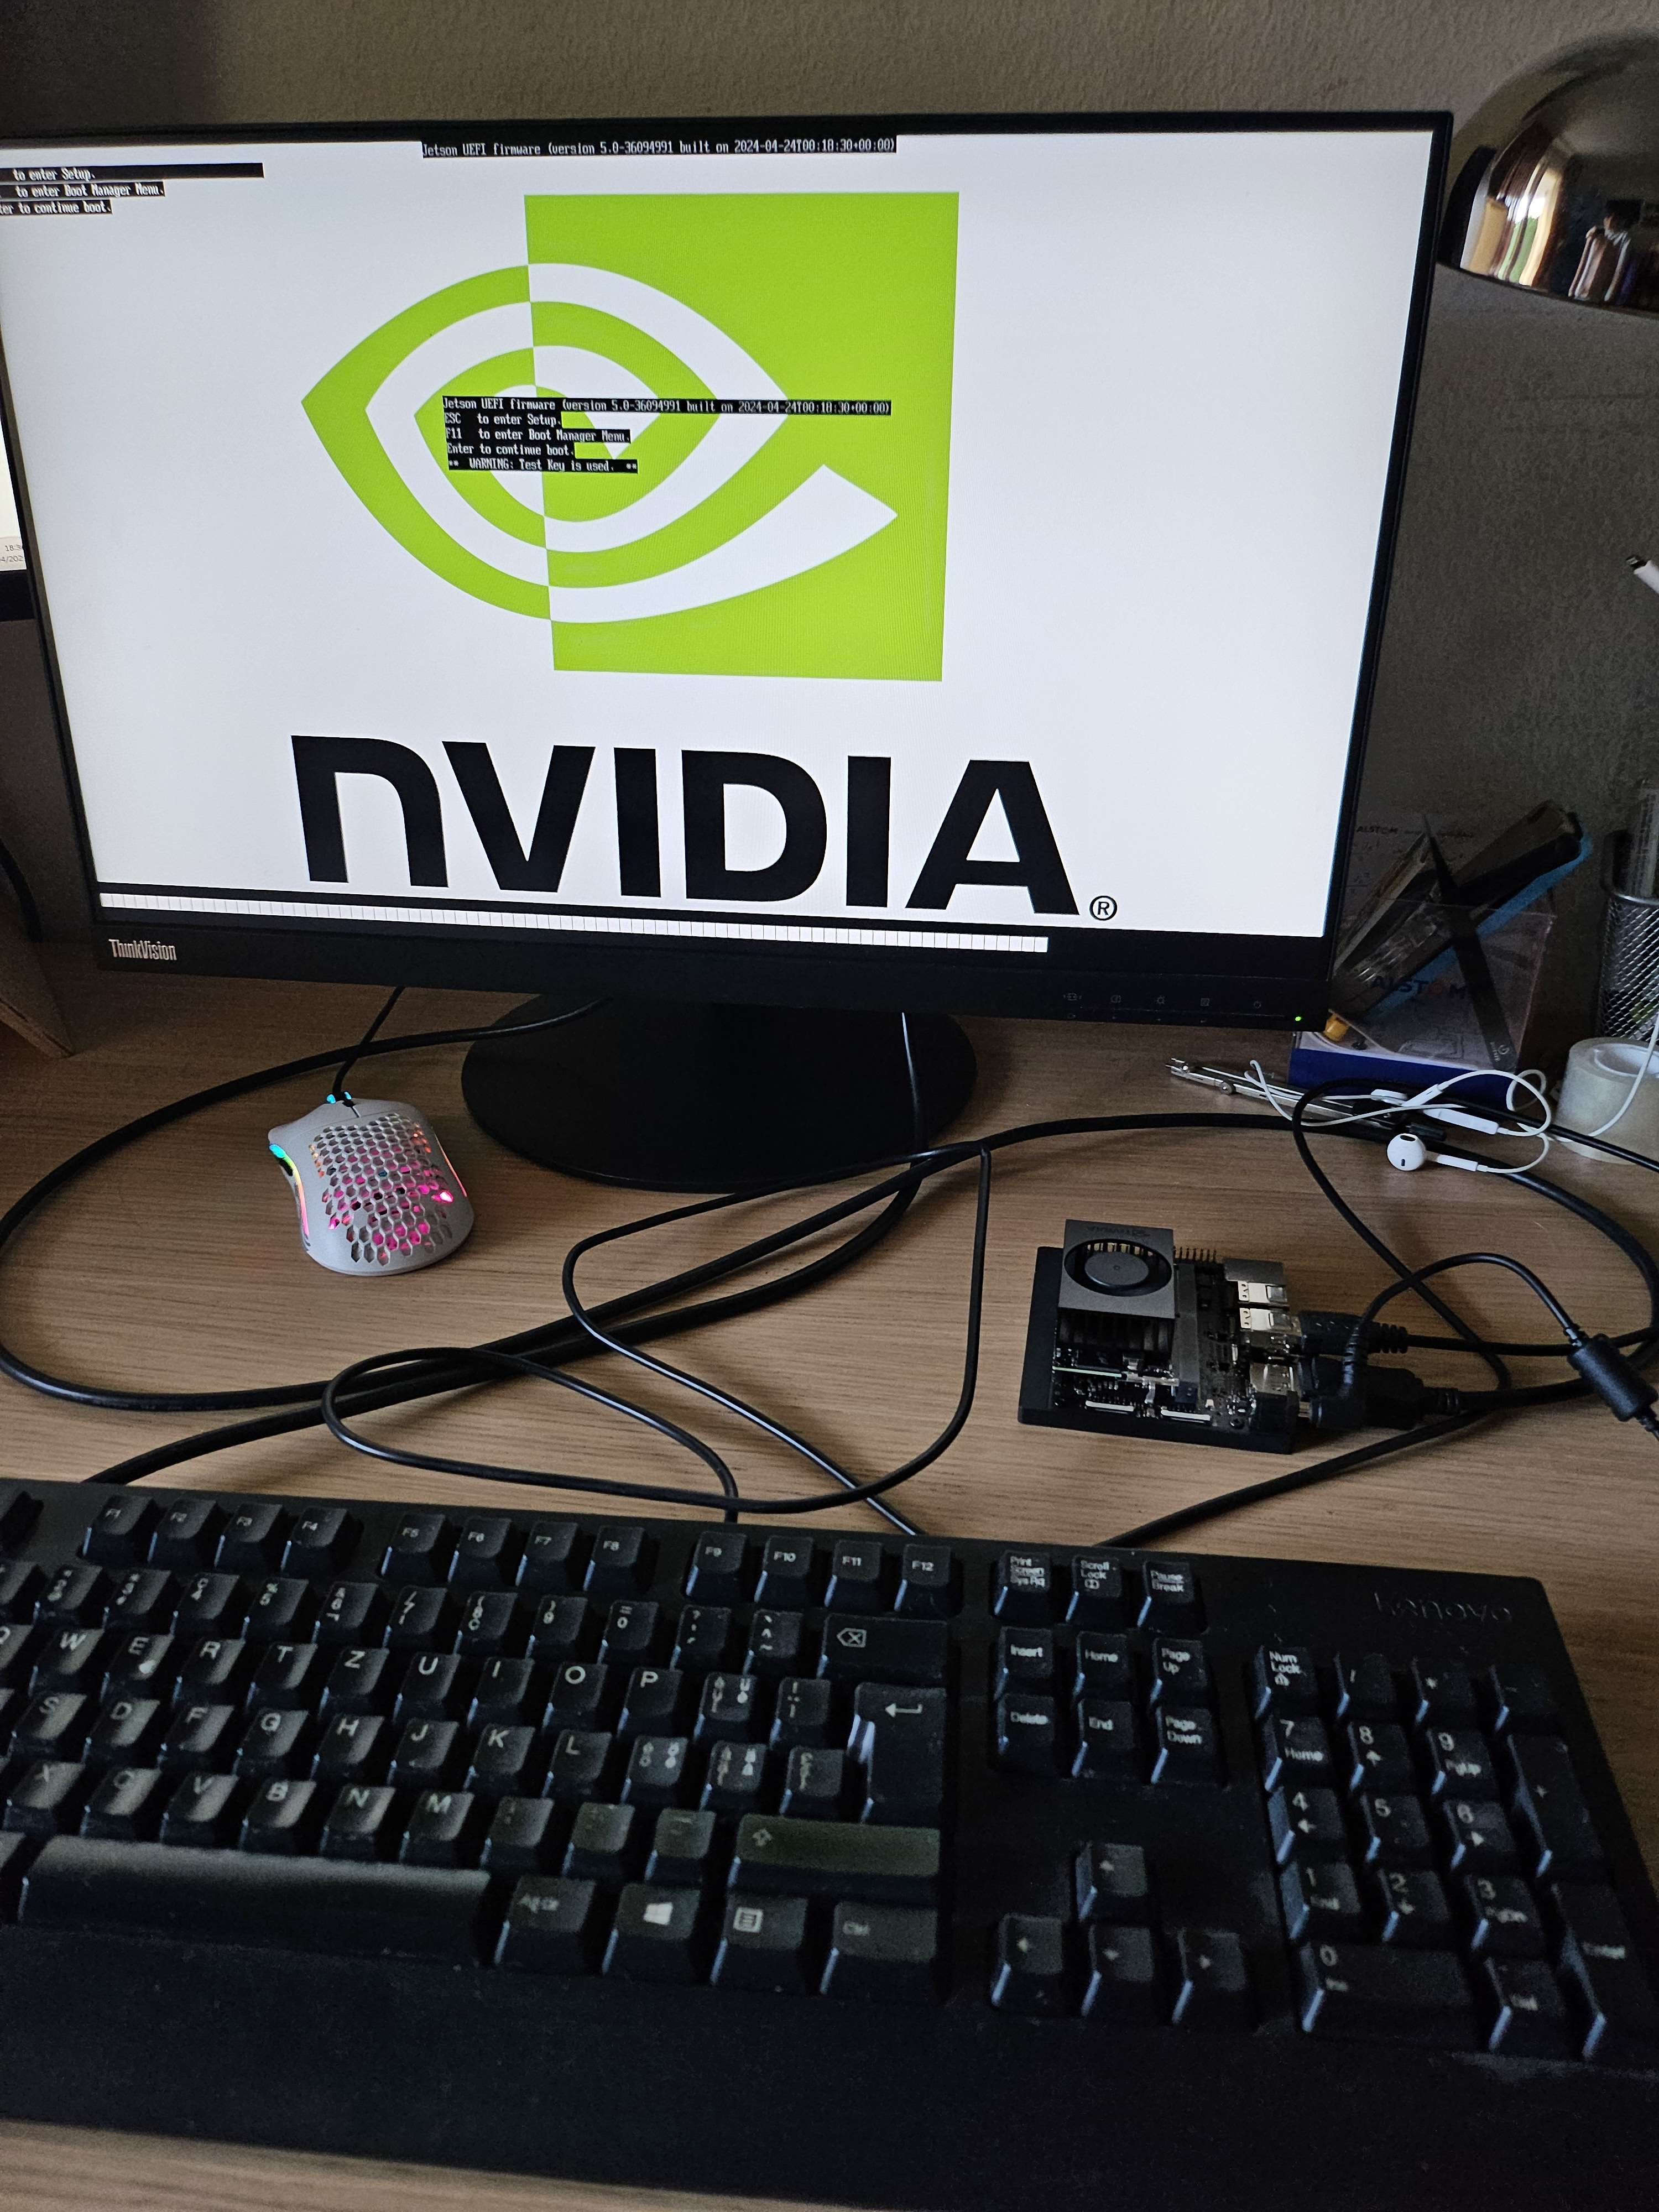
\includegraphics[width=0.5\paperwidth]{images/JetsonBoot.jpg}
    \caption{You can see the aformentioned Nvidia Jetson device booting up.}
    \label{fig:JetsonBoot}
\end{figure}

\newpage
\tableofcontents
\newpage




\subsection{Drop-Out}
When introducing a Drop-Out with an industry standard value of 0.3; contrary 
to the expectation of reducing over-fitting, which in some way is present, 
as the models aren't able to generalize beyond the training range, this has 
a negative effect on the model. The MSEs of models with Drop-out are higher 
then, the ones of the previous models without drop-out.
% https://github.com/AntonStantan/matura/blob/main/FNN_Heatmaps/DropOutComparison.png
%this is kinda wrong. Will explain later

\section{Recurrent Neural Network (RNN)}
\subsection{Introduction}
Recurrent Neural Networks (RNNs) work similar to FNNs with one key 
difference: There is a vector called the hidden-state. This vector contains 
information about previous inputs. The hidden-state of the previous 
time-step, in addition to the input of the current time-step, is fed into a 
model which computes the hidden-state of the present time-step. The output 
of each time-step is calculated by feeding the respective hiddenstate to a 
model.

\newpage
\textbf{ Numerical Visualization:}
\\

Let:
\begin{itemize}
    \item $x_t$: Input at time step $t$
    \item $h_t$: Hidden state at time step $t$
    \item $y_t$: Output at time step $t$
    \item $W_{xh}$: Weight matrix connecting input to hidden state
    \item $W_{hh}$: Weight matrix connecting previous hidden state to current hidden state (recurrent weights)
    \item $W_{hy}$: Weight matrix connecting hidden state to output
    \item $b_h$: Bias vector for the hidden layer
    \item $b_y$: Bias vector for the output layer
    \item $\sigma$: Activation function (commonly tanh or ReLU for the hidden state)
    \item $\sigma_{out}$: Activation function for the output (e.g. softmax for classification, or linear in our case of regression)
\end{itemize}



$$h_t = \sigma(W_{xh}x_t + W_{hh}h_{t-1} + b_h)$$

$$y_t = \sigma_{out}(W_{hy}h_t + b_y)$$



Useful sources for the creation of the first RNN prototype:
% https://www.ibm.com/think/topics/recurrent-neural-networks
% https://arxiv.org/pdf/1406.1827
% https://www.tensorflow.org/guide/keras/working_with_rnns
\newpage

\section{attention}

%https://arxiv.org/abs/1409.0473
%https://arxiv.org/abs/1508.04025
%https://www.tensorflow.org/api_docs/python/tf/keras/layers/Attention
\end{document}
